\section{Resultados}
\subsection{Función Transferencia de las Redes}
Una manera útil de pensar de una red es con un punto de vista basado en teoría de control. De esta forma, construimos una función de transferencia calculando la respuesta de la red a ciertas frecuencias. 
\begin{figure}[h!]
    \centering
    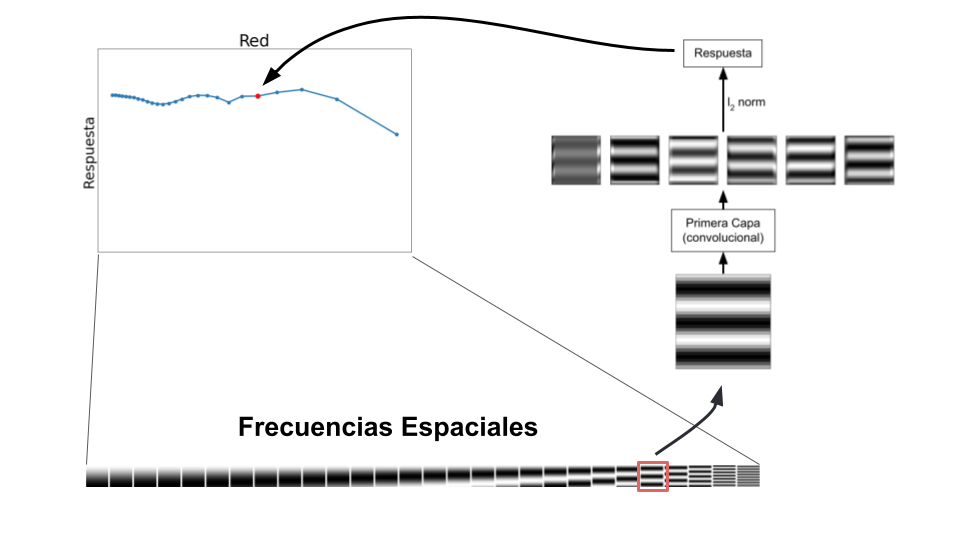
\includegraphics[width=\textwidth]{images/bode_diagrams/explanation_bode.png}
    \caption{stuff}
    \label{bode_explain}
\end{figure}

Así se puede ver las frecuencias a las que la red tiene mayor o menor sensibilidad.

\begin{figure}[h!]
    \centering
    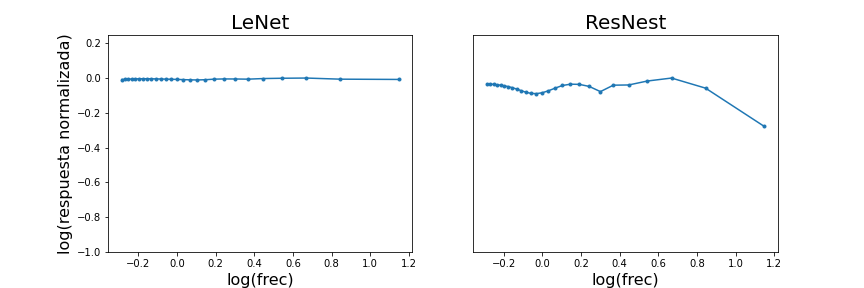
\includegraphics[width=\textwidth]{images/bode_diagrams/mnist_nets.png}
\end{figure}
\subsection{¿Qué hace la defensa de JPEG?}

Como vimos en la sección de compresión JPEG, cuando esta es aplicada a una imagen que ha sido sometida a un ataque adversario, los componentes de alta frecuencia se eliminan y, así como los humanos percibimos en menor medida dichos componentes, es posible que la red no logre distinguir el ataque perpetrado sobre la imagen, esto debido a que los ataques suelen tratarse de pequeñas cantidades de ruido o distorsión introducidos en la imagen y, al reducir la calidad de la misma, la red tiene más probabilidades de recuperar la clasificación original de la imagen. Esto se encuentra esquematizado en la Figura \ref{jpegexample}.

\begin{figure}[h!]
    \centering
    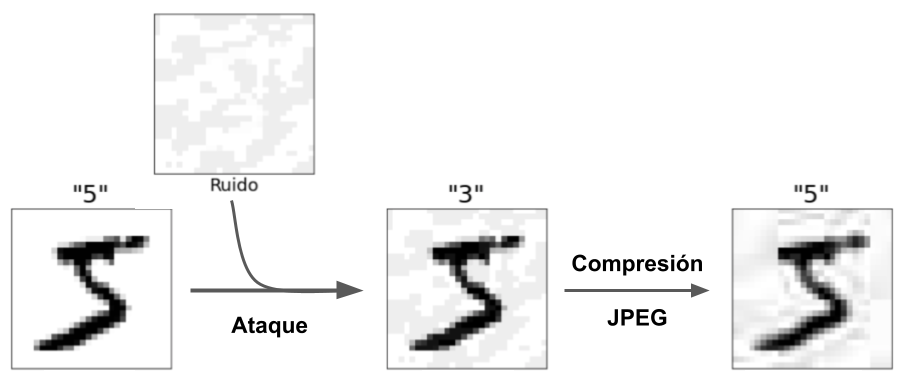
\includegraphics[width=0.8\textwidth]{images/jpeg/jpegdefense_example.png}
    \caption{La defensa JPEG radica en contrarrestar el ruido agregado por el ataque adversario al remover los componentes de alta frecuencia, que son los causantes de la falla en la clasificación de la red. En este ejemplo, el dígito 5 es clasificado como un 3 con el ruido del ataque, pero al hacer una compresión JPEG, la red clasifica correctamente al dígito como un 5.}
    \label{jpegexample}
\end{figure}

En la Figura \ref{jpeg_def} se muestra el resultado de nuestro entrenamiento de las redes LeNet y ResNet utilizando MNIST y el ataque FGSM con la norma $L_\infty$ para distintos niveles de compresión JPEG como defensa. Se observa que, efectivamente, conforme aumenta la compresión (disminuye la calidad), la precisión (accuracy) en la clasificación de las imágenes por parte de la red es mayor. Nótese que con ResNet la precisión decae más rápidamente conforme aumenta el épsilon.
\begin{figure}[h!]
    \centering
    \begin{subfigure}[b]{0.49\textwidth}
        \centering
        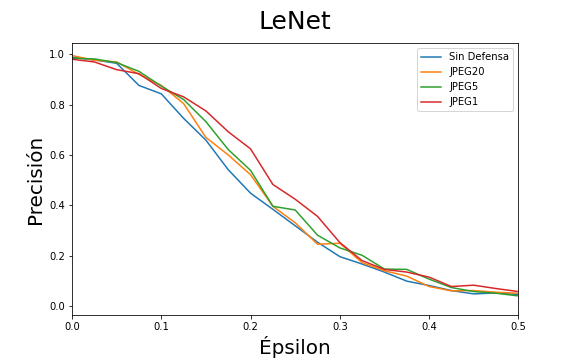
\includegraphics[width=\textwidth]{images/jpeg/jpegdefense_vs_epsilon_linear.png}
        \caption{Compresión JPEG contra FGSM usando LeNet}
    \end{subfigure}
    \begin{subfigure}[b]{0.49\textwidth}
        \centering
        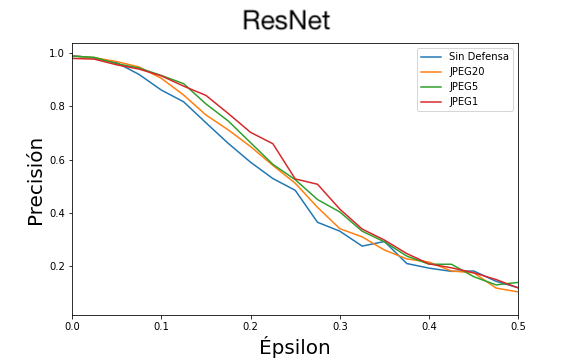
\includegraphics[width=\textwidth]{images/jpeg/jpegdefense_vs_epsilon_nonlinear.png}
        \caption{Compresión JPEG contra FGSM usando ResNet}
    \end{subfigure}
    \caption{Resultado de la compresión JPEG como defensa ante el ataque FGSM sobre MNIST}
    \label{jpeg_def}
\end{figure}
\pagebreak


{\LARGE \textbf{to do:}}
\begin{itemize}
    \item Carlini Wagner attack graphs
    \item JPEG defense graphs with cifar10
    \item Bode diagrams with jpeg conversion as first layer
    
    
\end{itemize}
\begin{figure}
    
\end{figure}
\animategraphics[autoplay,loop, width=0.48\linewidth]{5}{images/bode_diagrams/LeNet/}{1}{100}
\animategraphics[autoplay,loop, width=0.48\linewidth]{5}{images/bode_diagrams/ResNet/}{1}{100}
% \begin{subfigure}[t]{0.22\textwidth}
% \centering
%     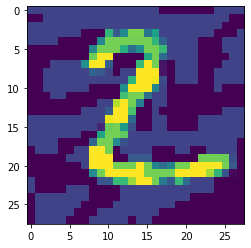
\includegraphics[width=\textwidth]{images/jpeg/fgsm_Le.png}
%     \caption{Sin compresión JPEG}
% \end{subfigure}
% \hspace{1em}
% \begin{subfigure}[t]{0.22\textwidth}
% \centering
%     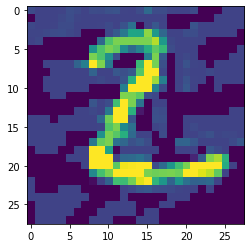
\includegraphics[width=\textwidth]{images/jpeg/fgsm_jpeg20_Le.png}
%     \caption{20\%}
% \end{subfigure}
% \hspace{1em}
% \begin{subfigure}[t]{0.22\textwidth}
% \centering
%     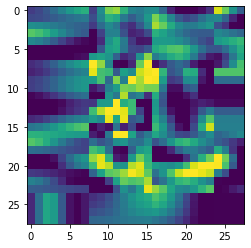
\includegraphics[width=\textwidth]{images/jpeg/fgsm_jpeg1_Le.png}
%     \caption{1\%}
% \end{subfigure}
% \caption{Ruido del ataque FGSM para distintas calidades en la compresión JPEG en el elemento \texttt{test[1]} de MNIST. En todos los casos, la red clasificó al 2 como un 7.}


% En la Figura \ref{Noise} se observa cómo el ruido generado por el ataque FGSM también se distorsiona conforme aumenta la compresión JPEG.



\subsection{Los efectos de Overfitting y Overparameterization}

Se ha sugerido que algunas propiedades de ciertas redes pueden contribuir a su susceptibilidad a los ataques adversarios. Por ejemplo, en el contexto de las imágenes médicas y sus redes respectivas, se propone que el overfitting y overparameterization pueden actuar de esa manera \cite{ma2020understanding}. El \textit{overfitting} ocurre cuando el modelo clasifica bien los datos de entrenamiento, pero no se generaliza tan bien, es decir, en los datos de validación tiene peor desempeño. \textit{Overparameterization} tiene lugar cuando hay tantos parámetros que la red es capaz de ``memorizar'' completamente los datos. Hicimos un pequeño análisis para probar esta hipótesis y no encontramos resultados que la apoyen. De hecho, con las redes que probamos, encontramos lo opuesto. En general, overfitting y overparameterization hacen que la red sea más robusta a los ataques adversarios (Figure \ref{overaparam_overfit}).

Para explorar el overfitting, cinco redes fueron entrenadas usado distintos numeros de épocas (epochs). Enre más épocas, más probabilidad de que la red haya sido sobreajustada. Para ver lo mismo con overparameterization, seis redes fuernon entrenadas con distinas cantidades de parámetros. Se le metieron un cierto número de capas (layers) adicionales directamente antes de la última. Cada capa adicional tenía 256 nodos. Así que, probamos redes con varios números de parámetros (Cuadro \ref{overparam_table}).

\begin{table}[h]
    \centering
    \begin{tabular}{|c|c|}
     \hline
     Red & Número de parámetros  \\ 
     \hline
     Normal & $61,706$  \\ 
     \hline
     2 Capas Adicionales & $150,978$  \\ 
     \hline
     4 Capas Adicionales & $282,562$  \\ 
     \hline
     6 Capas Adicionales & $414,146$  \\ 
     \hline
     10 Capas Adicionales & $743,106$  \\ 
     \hline
     20 Capas Adicionales & $1,335,234$  \\ 
     \hline
    \end{tabular}
    \caption{table}
    \label{overparam_table}
\end{table}

\begin{figure}[h]
    \centering
    \begin{subfigure}[b]{0.49\textwidth}
        \centering
        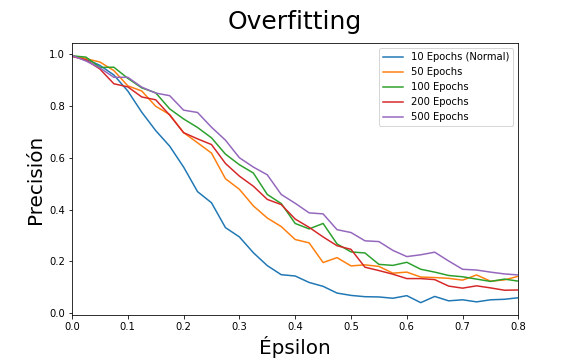
\includegraphics[width=\textwidth]{images/overfit_vs_attack.png}
        \caption{}
        \label{overfit}
    \end{subfigure}
    \begin{subfigure}[b]{0.49\textwidth}
        \centering
        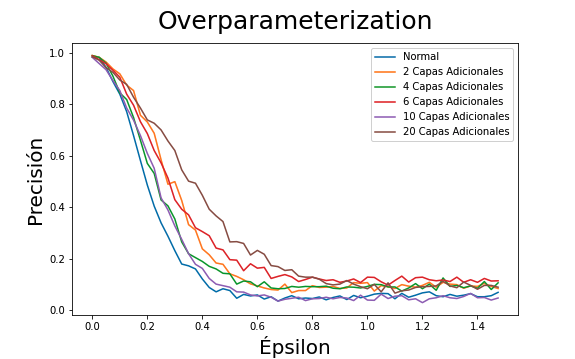
\includegraphics[width=\textwidth]{images/overparam_vs_attack.png}
        \caption{}
        \label{overparam}
    \end{subfigure}
    \caption{ a) El overfitting consiste en tener exceso de épocas. Aquí se observa que conforme aumenta el número de épocas, la precisión aumenta con respecto a cada épsilon. b) Overparameterization consiste en exceso de capas. En general, aumentar el número de capas aumenta la precisión.}
    \label{overaparam_overfit}
\end{figure}

\pagebreak
    
\subsection{Saliency}
\begin{itemize}
    \item Show figures from notebook of how adversarial noise attacks parts of the image that seem vulnerable (for example changing a 3$\to$8)
    \item Show Gradient-based localization of both image sets and how they change after adding adversarial noise\cite{Selvaraju_2019}
\end{itemize}
